% !TeX root = ./2020-21-COMP250-07-session-materials_screen.tex
\part{A selection of PCG techniques}
\frame{\partpage}

\pictureslideb{Combining hand-authored blocks}{spelunky_gen}{\url{http://tinysubversions.com/spelunkyGen2/}}

\begin{frame}{Perlin noise}
	\begin{columns}
		\begin{column}{0.4\textwidth}
			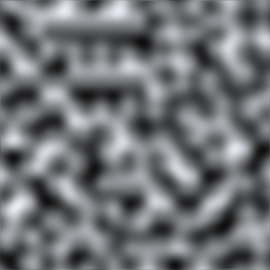
\includegraphics[width=\textwidth]{perlin}
		\end{column}
		\begin{column}{0.55\textwidth}
			\begin{itemize}
                \pause\item A ``smooth'' random number generator
                \pause\item Often used for terrain generation
                \pause\item 2D: use as height map
                \pause\item 3D: apply threshold to generate caves
			\end{itemize}
		\end{column}
	\end{columns}
\end{frame}

\begin{frame}{Fractals}
	\begin{columns}
		\begin{column}{0.4\textwidth}
			
\includegraphics[width=\textwidth]{mandelbrot}
		\end{column}
		\begin{column}{0.55\textwidth}
			\begin{itemize}
                \pause\item Some simple mathematical formulae can give rise to complex emergent structures
                \pause\item E.g.\ the Mandelbrot set: generated by iteration of the formula 
                    $$ z_{i+1} = z_i^2 + c $$
			\end{itemize}
		\end{column}
	\end{columns}
\end{frame}

\begin{frame}{L-Systems}
	\begin{columns}
		\begin{column}{0.4\textwidth}
			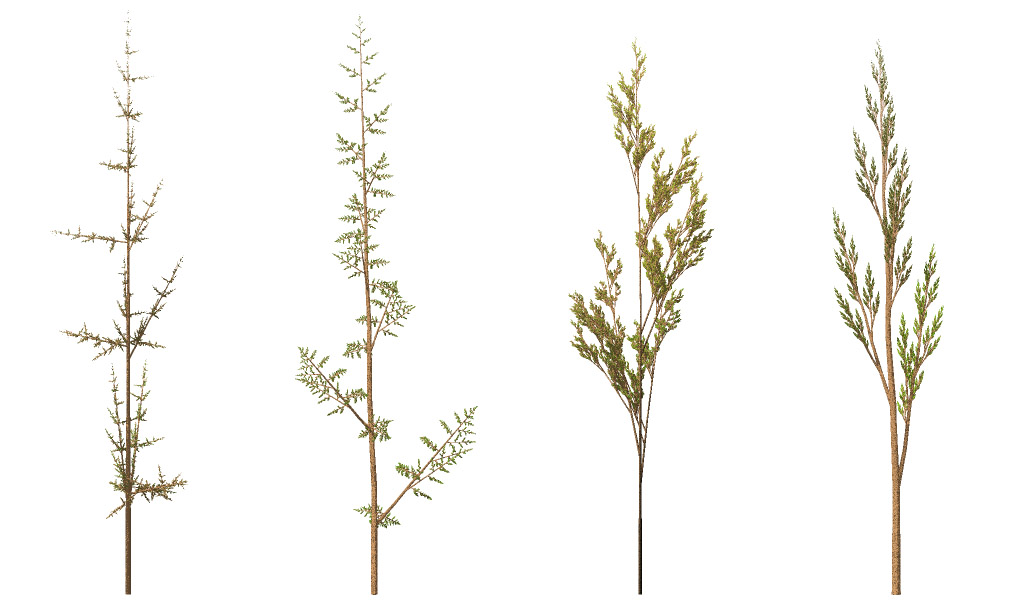
\includegraphics[width=\textwidth]{lsystem}
		\end{column}
		\begin{column}{0.55\textwidth}
			\begin{itemize}
                \pause\item Fractals based on repeated replacement of characters in a string representation
                \pause\item A simple model of plant growth
			\end{itemize}
		\end{column}
	\end{columns}
\end{frame}

\begin{frame}{Wave Function Collapse}
	\begin{columns}
		\begin{column}{0.4\textwidth}
			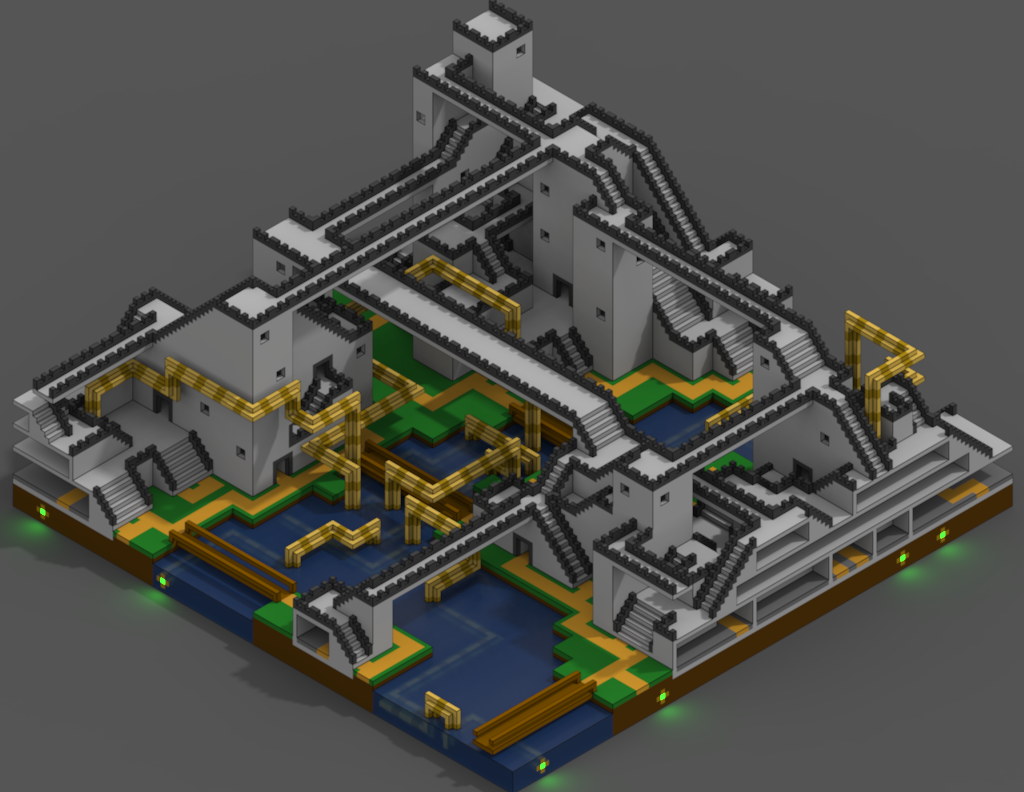
\includegraphics[width=\textwidth]{wfc}
		\end{column}
		\begin{column}{0.55\textwidth}
			\begin{itemize}
                \pause\item Places tiles (2D or 3D) based on constraints on which tiles can be adjacent
                \pause\item An example of \textbf{constraint solving} (similar to e.g.\ solving Sudoku)
			\end{itemize}
		\end{column}
	\end{columns}
\end{frame}

\begin{frame}{$n$-gram models}
	\begin{columns}
		\begin{column}{0.4\textwidth}
			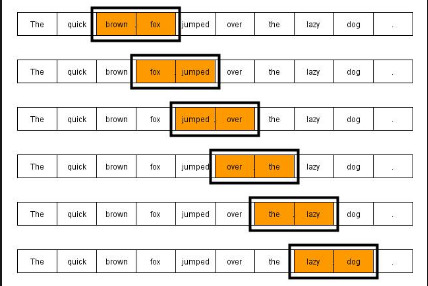
\includegraphics[width=\textwidth]{ngram}
		\end{column}
		\begin{column}{0.55\textwidth}
			\begin{itemize}
                \pause\item Gather frequency data for sequences of length $n$ in some training data
                \pause\item A basic form of machine learning
                \pause\item E.g.\ can train on letters to generate names
                \pause\item E.g.\ can train on words to generate (nonsense) text
                \pause\item E.g.\ can train on tiles to generate levels
			\end{itemize}
		\end{column}
	\end{columns}
\end{frame}

